\documentclass[longdoc, bigchapter, colorback,accentcolor=tud1c,12pt,numbersubsubsec]{tudreport}

\usepackage{hyperref}
\usepackage{subfigure}
\usepackage{epstopdf}
\usepackage[]{acronym}
\usepackage[utf8]{inputenc}
\usepackage[ngerman]{babel}


\usepackage{subfigure}


\usepackage{geometry}
\geometry{a4paper,left=25mm,right=20mm, top=1.5cm, bottom=1.5cm}
\usepackage{mathdesign}
\usepackage[]{subfigure}
\usepackage[]{graphicx}
\usepackage[square,numbers]{natbib}
\usepackage[]{amsmath}
%\usepackage{dsfont}
\usepackage{color}
\usepackage{booktabs}
\usepackage{verbatim}
\usepackage{listings}
\usepackage[ruled,chapter]{algorithm}
\usepackage[]{algorithmic}

\definecolor{red}{rgb}{1.,0.,0.}
%Eigene Befehle
\newcommand{\todo}{\textcolor{red}{\textbf{ToDo}}}
\newcommand{\image}{\textcolor{red}{\textbf{\\insert Image\\}}}
\newcommand{\quelle}{\textcolor{red}{\textbf{Quellenangabe}}}
\newcommand{\link}{\textcolor{red}{\textbf{Link}}}
\newcommand{\formel}{\textcolor{red}{\textbf{\\Formel\\}}}
\newcommand{\tabelle}{\textcolor{red}{\textbf{\\Tabelle\\}}}
% Pfad entlang dem die Bilder gesucht werden.
\graphicspath{{bilder/}}
%Kopfzeile
\linespread{1.2}                                 % Zeilenabstand
\setlength{\parindent}{6mm}                      % Absatzeinzug

\title{Sensitivität numerischer Vorhersagen des Wirkungsgrads von Hochdruckturbinen}
\subtitle{ADP | Keijo Buss, Dominik Henzel, Markus Degenhardt, Simon Lippert }
\subsubtitle{Betreuer: Faramarz Bakhtiari, Marius Schneider | Prof.Dr.-Ing.H.-P. Schiffer}
\institution{Fachbereich Maschinenbau\\Institut für Gasturbinen,\\ Luft- und Raumfahrtantriebe}
%Hier wird entweder ein Text für das Institut angewählt oder ein Logo
%\institution{Fachgebiet fŸr \\Numerische Berechnungsverfahren \\im Maschinenbau}
%\setinstitutionlogo[height]{CE}

%%% Untere Titelrückseite
\lowertitleback{%
	Keijo Buss, Dominik Henzel, Markus Degenhardt, Simon Lippert\\
	Studiengang: Computational Engineering M.Sc.\\ \\
	Thema: Sensitivität numerischer Vorhersagen des Wirkungsgrads von Hochdruckturbinen\\\\
	Eingereicht: 05.07.2017\\ \\
	%Rahmeninformationen
	Betreuer: Faramarz Bakhtiari\\
	\hspace*{4em} Marius Schneider\\\\
	Prof.Dr.-Ing.H.-P. Schiffer \\
	Fachgebiet Gasturbinen, Luft- und Raumfahrtantriebe\\
	Technische Universität Darmstadt\\
	Otto-Berndt-Straße 2\\
	64287 Darmstadt}
% %%%%%%%%%%%%%%%%%%% Hier beginnt das Dokument
\begin{document}
	\maketitle
	% Verzeichnisse mit römischen Seitenzahlen
	\cleardoublepage
	\pagenumbering{roman}
	\addcontentsline{toc}{chapter}{Abstract}
	%******  Abstract **************

\begin{abstract}
\setlength{\baselineskip}{11pt}
Die Zuverlässigkeit numerischer Vorhersagen der Wirkungsgrades von Turbinenstufen ist ein wichtiger Bestandteil diverser Forschungsaktivitäten wie Parameterstudien und Optimierungen. Mit zunehmender Komplexität der numerischen Modelle und der simulierten physikalischen Phänomene nimmt jedoch ach die Fehleranfälligkeit der numerischen Vorhersagen zu. Für eine sinnvolle Interpretation der numerischen Ergebnisse ist die Kenntnis der Einflussgrößen daher sehr wichtig. Um die eben genannte numerische Fehleranfälligkeit genauer zu untersuchen werden zwei Testfälle herangezogen. Zum Einen wird eine 1 1/2 Stufige Aachenturbine simuliert, des weiteren werden die Verbindungsstellen einzelner Domänen, sogenannte Interfaces, in einem einfachen Modell eines zweigeteilten Kanals untersucht. 

\begin{comment}
Die Ergebnisse von RANS sind heute immer weniger zufriedenstellend, da die verbesserte Rechenleistung für komplexere Verfahren ausreicht. LES dagegen ist für viele Fälle in der Industrie noch zu aufwändig und rechenintensiv. Eine hybride Variante, welche die Vorteile beider Verfahren kombiniert, soll diese Lücke dahingehend schließen, dass der benötigte Rechenaufwand den gegebenen Kapazitäten angeglichen wird.\\ \\
In diesem Sinne wird in dieser Arbeit eine DDES eines stationären und eines oszillierenden Zylinders bei einer Reynoldszahl von $Re = 10000$ mit dem Inhouse Strömungslöser FASTEST des Fachgebiets Numerische Berechnungsverfahren der TU Darmstadt durchgeführt. Als Turbulenzmodell wird das $\zeta$-$f$-Turbulenzmodell nach Hanjali\'{c} (2004)  verwendet. Ein besonderes Augenmerk wird auf die Entwicklung des Auftriebs- und Widerstandsbeiwertes in Abhängigkeit der Oszillationsfrequenz des Zylinders gelegt. Für das Auswerten der Ergebnisse stehen Experimente, insbesondere von Gopalkrishnan (1993) und eine DNS von Dong und Karniadakis (2005) , an der sich der Simulationsaufbau orientiert, zu Verfügung. Die in dieser Arbeit berechneten Werte der DDES stimmen gut mit diesen vorliegenden Ergebnissen aus Experiment und DNS überein.
\setlength{\baselineskip}{13.2pt}
\end{comment}

\end{abstract}
	\include{eid} 
	\tableofcontents

	
	% Eigentlicher Text mit arabischen Seitenzahlen
	\cleardoublepage
	\pagenumbering{arabic}
	\setcounter{page}{1}
	%Einbinden der einzelnen Kapitel
	%\chapter{Beispiele}
Test

\section{Beispielabbildung}
\begin{figure}
	\centering
	\label{simaufbau}
	\includegraphics[width=0.7\textwidth,angle=90]{screen.eps}
	\caption{Anordnung des umströmten Zylinders}
\end{figure}

\section{Beispieltabelle}
Beispieltabelle \ref{simaufbaufreqs}

\begin{table}[H]
	\caption{Unterschiedliche Frequenzen des oszillierenden Zylinders}
	\centering
	\begin{tabular}{l l l l}
		\hline
		Fall&$Y_0/d$&$f_0 d/U_0$& $f_0$\\ \hline
		M1 & 0,3 & 0,14& $2,205\text{Hz}$\\
		M2 & 0,3 & 0,17& $2,677\text{Hz}$\\
		M3 & 0,3 & 0,19& $2,992\text{Hz}$\\
		M4 & 0,3 & 0,21& $3,307\text{Hz}$\\
		M5 & 0,3 & 0,23& $3,622\text{Hz}$\\
		M6 & 0,3 & 0,25& $3,937\text{Hz}$\\ \hline
	\end{tabular}
\label{simaufbaufreqs}
\end{table}
\section{Beispielformel}
Beispielformel nach \cite{dong2005dns}
\begin{align}
x &= \\
y &= \\
z &= 0 - 0,0254 \pi.  
\end{align}

	%\include{einleitung}
	\chapter{Vorgehen}
In diesem Kapitel soll das Vorgehen zur Erstellung dieser Arbeit und zur Erlangung der vorgestellten Ergebnisse aufgezeigt werden. \\
Der Startpunkt der Arbeit ist ein Geometriemodell der 1 1/2 Stufigen Aachenturbine. Darauf aufbauend wurden erste Test-Simulationen durchgeführt, um sich mit der Thematik und der verwendeten Software vertraut zu machen. Die nächste Aufgabe besteht darin ein geeignetes Gitter für die endgültigen Berechnungen und Auswertungen zu finden. Hierbei wird zunächst der strukturierte Vernetzer AutoGrid von Numeca verwendet.\\
Anschließend wird ein Augenmerk auf die Verbindungsstellen der einzelnen Domänen, Interfaces, gelegt. Hierzu dient ein einfaches Kanalmodell, bestehend aus einem stationären Kanal gefolgt von einem rotierenden Kanal, mit Ähnlichen Abmessungen der Aachenturbine. Die Geometrieerstellung erfolgt mit Siemens NX, die Netzgenerierung mittels ANSYS ICEM CFD.\\ 
Die Auswerung der einzelnen Größen erfolgt mit MATLAB, hierfür dient eine während dieser Arbeit entwickelte Applikation zum einfacheren Einlesen der Ergebnisdaten und deren Visualisierung.    

\section{Aufbau der Arbeit}
\todo
	\chapter{Grundlagen}
In diesem Kapitel wird zu Beginn erläutert, wo sich die Turbine im Strahltriebwerk befindet und welche Aufgaben diese hat. Danach werden die verschiedenen Möglichkeiten zur Berechnung des Wirkungsgrades für Turbinen vorgestellt. Diese werden im Rahmen der Simulation der Aachen-Turbine getestet und die resultierenden Wirkungsgrade miteinander verglichen.

\section{Turbine}
Ein einfaches Strahltriebwerk besteht aus den folgenden Komponenten: Einlauf, Verdichter, Brennkammer, Turbine, Düse. Die Turbine befindet sich im Flugzeugtriebwerk also hinter der Brennkammer und dient dem Antrieb des Verdichters und der Hilfsaggregate. Sie ist eine adiabate, verlustbehaftete Arbeitsmaschine. In der Turbine wird die Strömung beschleunigt, entspannt und ihr dabei Leistung entzogen. Da es sehr schwierig ist, die gesamte Entspannung innerhalb einer einzigen Stufe bestehend aus Leitrad (Stator) und Laufrad (Rotor) durchzuführen, werden oft mehrere Stufen hintereinandergeschaltet. In der Regel herrschen am Turbineneintritt sehr hohe Temperaturen von bis zu 1800K vor, daher ist eine ausreichende Kühlung der Schaufeln unerlässlich.


\begin{figure}[htbp]
	\centering
	\includegraphics[width=0.8\textwidth]{RRTurbine_comment.png}
	\caption{Rolls-Royce Trent 500 Triebwerk \cite{RRFlickr}} \label{fig:RRTurbine}
\end{figure} 

\section{Wirkungsgradberechnung}
\label{sec:wgberechnung}
Betrachtet man den Kreisprozess der Gasturbine - den Joule-Prozess - findet in der Turbine eine isentrope Entspannung bzw. Expansion statt. Aus dem ersten Hauptsatz der Thermodynamik ergibt sich mit adiabater Zustandsänderung und unter Vernachlässigung der Reibungsverluste die von der Turbine an den Verdichter abgegebene Leistung zu
\begin{equation}
\label{eq:leistungTurbine}
P = \dot m (h_{t5} - h_{t4})
\end{equation}
wobei $h_{t5}$ die Totalenthalpie am Turbinenaustritt und $h_{t4}$ die Totalenthalpie am Turbineneintritt ist. 



%__________________________
\subsection{Wirkungsgrad allgemein}

Wie in Abb. \ref{fig:hsTurbine} zu sehen, ergibt sich der isentrope Wirkungsgrad aus dem Verhältnis der verlustbehafteten und der isentropen Enthalpiedifferenz bzw. dem Verhältnis der Turbinenleistungen zu:

\begin{equation}
\label{eq:leistungTurbine}
\overline{\eta}_{t} = \frac{h_{t5} - h_{t4}}{\overline{h}_{t5} - h_{t4}} =  \frac{P}{ \overline{P}} 
\end{equation}

\begin{figure}[htbp]
	\centering
	\includegraphics[width=0.5\textwidth]{hsTurbine.png}
	\caption{h-s-Diagramm der Turbine} \label{fig:hsTurbine}
	
\end{figure} 

Oder umformuliert mit der isentropen Totalenthalpiedifferenz dargestellt durch $\Delta H_{t_{is}} = \overline{h}_{t5} - h_{t4}$ zu:
\begin{equation}
\label{eq:wgallgemein}
\eta =\frac{P}{\Delta H_{t_{is}}}
\end{equation}

Die isentrope Enthalpiedifferenz $\Delta H_{t_{is}}$ wird nach
\begin{equation}
\label{eq:wgnenner}
\Delta H_{t_{is}} = \dot m \cdot c_p \cdot T_{t_{inlet}} \cdot \left[ \left( \frac{p_{t_{outlet}}}{p_{t_{inlet}}}\right)^\frac{\gamma-1}{\gamma}-1\right]
\end{equation}
mit dem Massenstrom $\dot m$, der spezifischen Wärmekapazität bei konstantem Druck $c_p$ (siehe Berechnungsweise Abschnitt \ref{subsec:spezWK}), der Totaltemperatur am Inlet $T_{t_{inlet}}$, dem Totaldruck am Inlet $p_{t_{inlet}}$, dem Totaldruck am Outlet $p_{t_{outlet}}$ und dem Isentropenexponenten $\gamma$ berechnet.\newline 
Im folgenden Abschnitt werden verschiedene Definitionsmöglichkeiten für die erzeugte Leistung $P$ vorgestellt.
%__________________________
\subsection{Erzeugte Leistung}
\label{sec:wirkungsgrade}
Die erzeugte Leistung $P$ im Zähler der Gleichung \ref{eq:wgallgemein} für den Wirkungsgrad  lässt sich unter anderem mit einer der drei folgenden Gleichungen berechnen:\newline
Mit Hilfe der tatsächlichen Totaltemperaturdifferenz $\Delta T_t$ und der spezifischen Wärmekapazität $c_p$ nach:
\begin{equation}
\label{eq:wgzaehlertt}
P_{\Delta T_t} = \dot m \cdot c_p \cdot \Delta T_t = \dot m \cdot c_p \cdot \left( T_{t_{inlet}}-T_{t_{outlet}} \right),
\end{equation}
mit Hilfe der Totalenthalpie am Inlet $h_{t_{inlet}}$ und Outlet $h_{t_{outlet}}$, welche direkt aus ANSYS CFX entnommen wird, nach:
\begin{equation}
\label{eq:wgzaehlerht}
P_{\Delta h_t} = \dot m \cdot \Delta h_t = \dot m \cdot \left( h_{t_{inlet}}-h_{t_{outlet}} \right)
\end{equation}
oder mit Hilfe des Momentes $M_{Rotor}$ um die Rotationsachse an Schaufel und Hub des Rotors, der Anzahl Rotoren $N_{Rotor}$ und der Winkelgeschwindigkeit des Rotors $\omega_{Rotor}$ nach:
\begin{equation}
\label{eq:wgzaehlertorque}
P_{torque} = M_{Rotor} \cdot N_{Rotor} \cdot \omega_{Rotor}
\end{equation}
Da auch die Berechnung der spezifischen Wärmekapazität $c_p$ aus den Gleichungen \ref{eq:wgnenner} und \ref{eq:wgzaehlertt} Einfluss auf den Wirkungsgrad haben kann, wird im kommenden Abschnitt näher auf dessen Definition eingegangen.

\subsubsection{Spezifische Wärmekapazität}
\label{subsec:spezWK}
Die spezifische Wärmekapazität bei konstantem Druck $c_p$ ist eine temperaturabhängige Größe. Wenn die Temperaturdifferenz zwischen In- und Outlet sehr groß ist, verändert sich $c_p$ zwischen In- und Outlet wesentlich und kann somit nicht mehr als konstant angenommen werden. Die temperaturabhängige Wärmekapazität $c_p$ lässt sich mit dem folgenden Polynom in Abhängigkeit der Temperatur $T$ berechnen, zu sehen in Abbilgung \ref{fig:cpPlot}.  
\begin{equation}
\label{eq:cppolynom}
c_p = \frac{a\cdot T^4-b\cdot T^3+c\cdot T^2-d\cdot T+e}{f}\frac{J} {kg \cdot K}
\end{equation}
Die Konstanten $a$ bis $f$ sind der folgenden Tabelle \ref{tab:cpparameter} zu entnehmen.
\begin{table}[H]
\centering
\caption{Konstanten für die Berechnung von $c_p$} \label{tab:cpparameter}
\begin{tabular}{ c| c|c|c|c|c}
$a$&$b$&$c$&$d$&$e$&$f$\\
\hline
$0.12934K^{-4}$&$596.633K^{-3}$&$933833K^{-2}$&$373,61\cdot10^6K^{-1}$&$105,01\cdot10^{10}$&$10^9$\\
\end{tabular}

\end{table}

\begin{figure}[htbp]
	\centering
	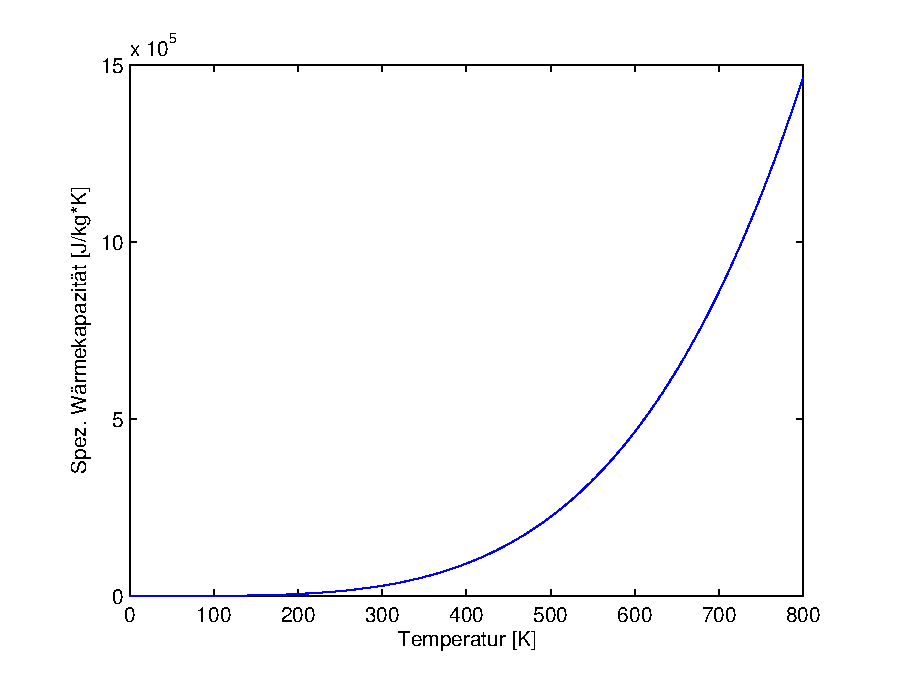
\includegraphics[width=0.8\textwidth]{cp_Plot.eps}
	\caption{Spez. Wärmekapazität temperaturabhängig} \label{fig:cpPlot}
	
\end{figure} 

Bei der Berechnung der isentropen Enthalpiedifferenz $\Delta H_{t_{is}}$ aus Gleichung \ref{eq:wgnenner} wurde $c_p$ nach Gleichung \ref{eq:cppolynom}
\begin{itemize}
	\item separat am In-/Outlet: $c_{p_1} = c_p(T_1)\, ;\, c_{p_3} = c_p(T_3)$,
	\item in Abhängigkeit der isentropen Temperatur im Outlet: $c_{p_3}^* = c_{p_3}(T_{3_{is}})$,
	\item aus dem arithmetischen Mittel der beiden Größen: $\bar{c_p} = \frac{c_{p_1} + c_{p_3}}{2}\, ;\, \bar{c_p^*} = \frac{c_{p_1} + c_{p_3}^*}{2}$
	
\end{itemize}
berechnet um den Einfluss der Berechnungsweise von $c_p$ auf die Berechnung des Wirkungsgrades zu analysieren.\\

Die verschiedenen Wirkungsgraddefinitionen in Abschnitt \ref{sec:wirkungsgrade} und Berechnungsweisen von $c_p$ wurden in CFX implementiert und miteinander verglichen. Das Ergebnis dieses Vergleichs wird im nächsten Abschnitt dargestellt.
%__________________________

\begin{comment}
\section{Wirkungsgrade bei der Aachen-Turbine}
\label{sec:wgaachen}
Bei der Aachen-Turbine ergaben sich je nach Berechnungsart folgende Werte für den Wirkungsgrad:
\begin{table}[H]
\centering
\caption{Wirkungsgrad bei der Aachen-Turbine}
\begin{tabular}{ c| c}
Berechnungsformel & $\eta$ \\
\hline
$\eta_{\Delta T_t}$ mit $c_p$ konstant& 86\% \\
$\eta_{\Delta T_t}$ mit $c_p(T)$& 86\% \\
$\eta_{\Delta h_t}$& 87\% \\
$\eta_{torque}$& 85\% \\
\end{tabular}
\label{tab:wgaachen}
\end{table}
Es ist zu sehen, dass .....
\todo
\end{comment}




%%% Local Variables: 
%%% mode: latex
%%% TeX-master: "main"
%%% End: 



 %Dominik Keijo eingefügt
	\chapter{Aachen-Turbine}
\label{cha:aachen}
Zur Analyse der verschiedenen Wirkungsgraddefinitionen wurde eine sogenannte Aachen-Turbine, das heißt eine Turbine mit einfachen Schaufeln ohne Krümmung in Radialrichtung simuliert. In diesem Kapitel wird zunächst die Geometrie und die durchgeführte Gitterstudie vorgestellt. Danach werden die ermittelten Wirkungsgrade miteinander verglichen und Unterschiede vorgestellt.
\section{Geometrie}
\label{sec:aachengeo}
  \begin{figure}[htbp]
	\centering
	\label{fig:imgAachenTurbine}
	\includegraphics[width=0.7\textwidth]{AachenTurbine_trans.png}
	\caption{Aachen-Turbine}
\end{figure} 
Die verwendete Geometrie basiert auf der Aachen-Turbine, die auch in den Untersuchungen von TO DO verwendet wurde. Es wurden dabei nur anderthalb Stufen berechnet, um den Rechenaufwand der Simulationen gering zu halten und der Vergleich der Wirkungsdefinitionen auch für diesen Aufbau möglich ist. Die Geometrie der Aachen-Turbine mit Gitter ist in der Abbildung \ref{fig:aachengebiet} zu sehen. TODOTODOTODO
\begin{figure}[H]
\includegraphics[width=\textwidth]{aachenmitgitter.png}
\caption{Eine dreidimensionale Ansicht der Aachen-Turbine mit Gitter.}
\label{fig:aachengebiet}
\end{figure}
Die Aachen-Turbine besteht aus zwei Statoren und einem Rotor. Der vordere Teil ist der erste Stator mit Einstrom, der mittlere Teil ist der Rotor und der hintere Teil ist der zweite Stator mit Ausstrom. Die Grenzen an den Seiten stellen Shroud und Hub dar. Oben und unten herrschen periodische Randbedingungen. Die Statoren sind jeweils durch ein Interface mit dem Rotor verbunden. Die Anzahl an Blades in Stator und Rotor sind der folgenden Tabelle \ref{tab:aachenabmessungen} zu entnehmen.
\begin{table}[H]
\centering
\label{tab:aachenabmessungen}
\caption{Bladeanzahl im Stator und Rotor}
\begin{tabular}{ c| c}
Anzahl Blades im Stator&Anzahl Blades im Rotor\\
\hline
36&41\\
\end{tabular}
\end{table}
Im folgenden Abschnitt wird der gewählte Betriebspunkt näher beschirieben.
%________________________________________________________
\section{Betriebspunkt}
\label{subsec:aachensetup}
Als Betriebspunkt wurden die Randbedingungen der Analyse der Aachen-Turbine von TO DO übernommen. Diese sind der folgenden Tabelle \ref{tab:aachensetup} zu entnehmen. Im 
\begin{table}[H]
\centering
\caption{tab:aachensetup}
\begin{tabular}{ c| c| c| c}
$T_{t_{Inlet}}$&$p_{t_{Inlet}}$&$Massenstrom$&$\omega_{Rotor}$\\
\hline
305&152.000&2&3500\\
\end{tabular}
\end{table}
In den verschiedenen Aufgabenteilen wurden die Eintrittsbedingungen jedoch auch verändert, um zum Beispiel den Einfluss inhomogener Eintrittsbedingungen oder höherer Temperaturen zu untersuchen.

\section{Strukturiertes Gitter}
Im Folgenden wird beschrieben, wie das strukturierte Netz der Aachen-Turbine erstellt wurde. Da das Netz die numerische Konvergenz der Lösungsverfahren, Qualität der Lösung, Auflösung und damit auch den Diskretisierungsfehler beeinflusst, ist ein gutes Netz von großer Bedeutung. Deshalb wurde eine Netzstudie - basierend auf einem Referenzgitter – durchgeführt und anschließend das bestmögliche Netz in Bezug auf Qualität vs. Rechenaufwand ausgewählt. Es war außerdem im Fokus, wie sich Netze unterschiedlicher Topologie hinsichtlich der erforderlichen Netzauflösung unterscheiden.

\subsection{Erstellung des Gitters}

Zunächst wurde das Referenzgitter erstellt. Dazu wurde die Geometrie der Aachen-Turbine mittels des strukturierten Multi-Block Netzgenerators AutoGrid5 vernetzt. Dieser ist speziell für die Vernetzung von Turbomaschinen ausgelegt. 
Das zur Verfügung stehende CAD-Modell der Aachen-Turbine die 1,5 Stufen zusammenhängend beinhaltete, wurden zu Beginn jeweils einzelne Gitter für Stator 1, Rotor und Stator 2 erzeugt, um diese später in CFX verwenden zu können. Hierbei wurde jeweils erst ein Vernetzungsdurchlauf basierend auf den voreingestellten Standardwerten durchgeführt und anschließend manuell optimiert. Für eine ausreichend gute Netzqualität dürfen bestimmte Netzkriterien nicht verletzt werden. Andernfalls kann es sein, dass der Diskretisierungsfehler steigt und die Lösung nicht oder nur schlecht konvergiert.
\begin{itemize}
	\item Keine negativen Kontrollvolumen
	\item Kleinster Winkel einer Zelle $> 20^\circ$
	\item Expasion ratio (Volumenverhältnis benachbarter Zellen) $< 3$
	\item Aspect ratio (Verhältnis längster zur kürzester Seite einer Zelle) $< 1000$ 
\end{itemize}
Variiert wurden die Anzahl und die Verteilung der Zellen in der S1-Ansicht. Diese stellt einen Querschnitt durch die Schaufel dar. In radialer Richtung wurde die Zellverteilung im „flowpath“ angepasst. 

\subsection{Spaltverfeinerung}

Zur Bestimmung der Gitterauflösung im Spalt des Rotors wurde zudem die Anzahl der Zellen im Spalt variiert. Es stellte sich heraus, dass im Vergleich zum ursprünglichen Gitter mehr Zellen hinzugefügt werden mussten, da die Auflösung nicht fein genug war und Änderungen, wie z.B. Spaltwirbel im Vergleich zur gröberen Auflösung nicht aufgelöst wurden. In den Abbildungen \ref{effSpalt1} und \ref{effSpalt15} ist die Gitterstudie für den Spalt mit 1 und 1,5 Stufen dargestellt. Als Ergebnis der Spaltverfeinerung wurde festgestellt, dass das Gitter mit der dreifachen Verfeinerung des ursprünglichen Spalts geeignet ist, da kaum noch ein Unterschied zum nächst feineren Gitter zu sehen ist und die Zellenanzahl trotzdem nicht zu groß ist.


\begin{figure}[H]
	\centering
	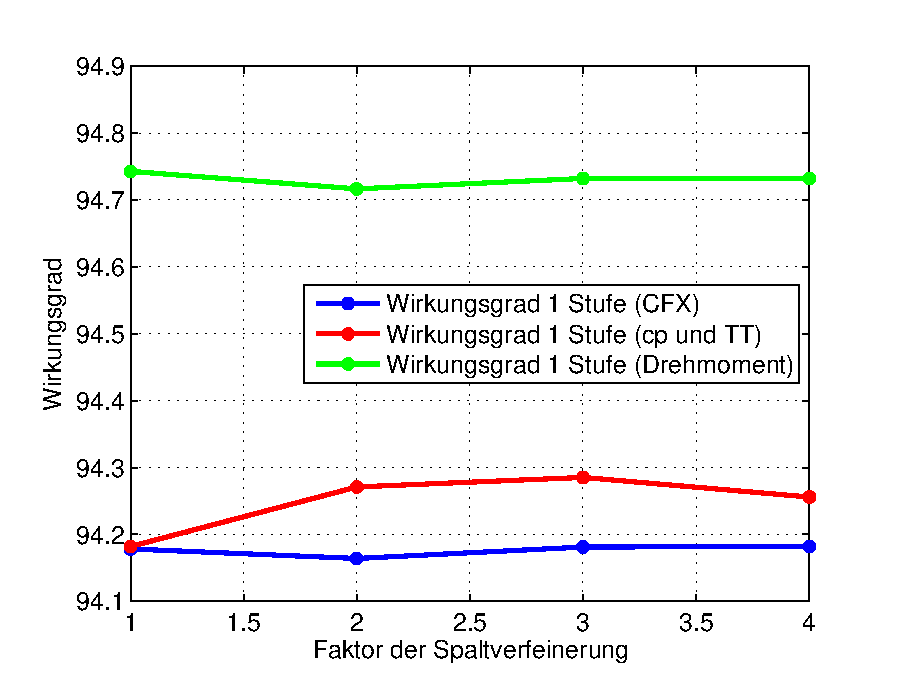
\includegraphics[width=0.7\textwidth]{efficiencySpalt1Stufe.eps}
	\caption{Gitterstudie des Spalts für eine Stufe} \label{effSpalt1}
\end{figure}

\begin{figure}[H]
	\centering
	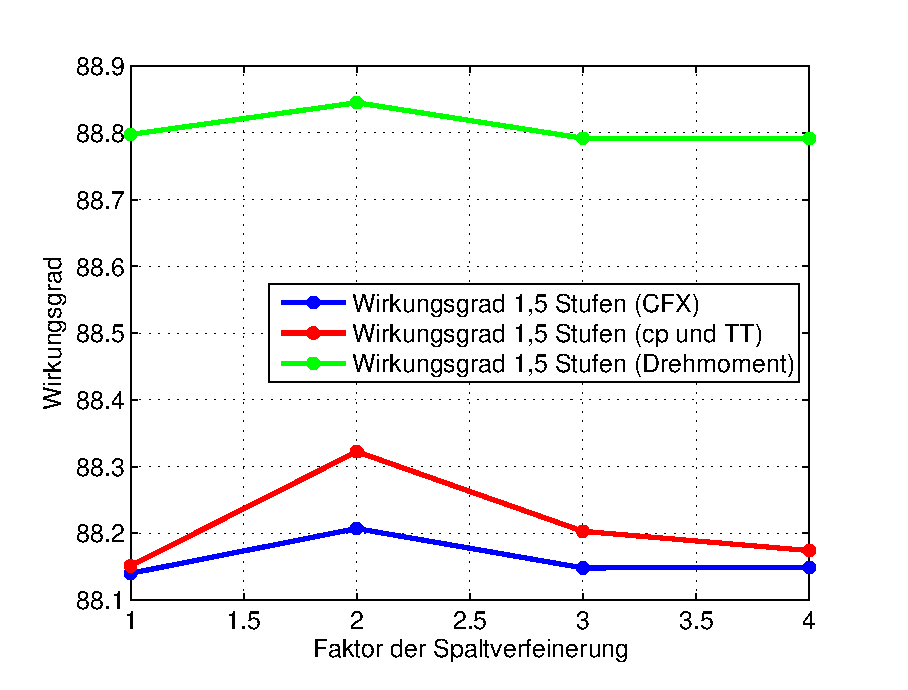
\includegraphics[width=0.7\textwidth]{efficiencySpalt15Stufen.eps}
	\caption{Gitterstudie des Spalts für 1,5 Stufen} \label{effSpalt15}
\end{figure}

\subsection{Einstellen der Grenzschichtdicke}
Der dimensionslose Wandabstand $y^+$ wurde iterativ bestimmt. Um das korrekte $y^+$ zu bestimmen, wurden die Werte in AutoGrid für den Wandabstand sowohl auf der Schaufeloberfläche im S1-Layer, als auch an Nabe und Gehäuse variiert.  Nach Bestimmen des Wandabstandes wurde eine Simulation in CFX durchgeführt und anschließend die Verteilung des $y^+$-Wertes über das Simulationsgebiet visualisiert und ausgewertet. Als finalen Wandabstand wurde für den Rotor $2\cdot 10^{-6}\text{m}$ im Flowpath an Nabe und Gehäuse und $1.5\cdot 10^{-6}\text{m}$ am Blade ermittelt. Ein Überblick der Werte ist in Tabelle \ref{cellWidths} zu sehen. Über das komplette Simulationsgebiet liegen die $y^+$-Werte in einem Bereich von $0.3 \leq y^+ \leq 3$. Da nur wenige Einstellparameter zur Beeinflussung dieses Wertes in AutoGrid vorhanden sind, ist dieser Wertebereich zufriedenstellend, zumal die Mehrheit der Werte im Bereich von $0.7 \leq y^+ \leq 1.2$  liegt, wie in Abb. \ref{imgYplusWerte} zu sehen ist. 

\begin{table}[H]
\centering
\begin{tabular}[t]{cccc}
\toprule
 Cell width in [m] & Stator1 & Rotor & Stator2  \\
\midrule
Cell width at Hub & $2.7e{-06}$ & $2e{-06}$ & $1.4e{-06}$\\
Cell width at Shroud & $2.7e{-06}$ & $2e{-06}$ & $1.4e{-06}$ \\
Cell width at Wall (Blade) & $1.56e{-06}$ & $1.5e{-06}$ & $1.7e{-06}$ \\
\bottomrule
\end{tabular}
\caption{Zellgrößen an der Wand für Rotor und die Statoren} \label{cellWidths}
\end{table}

\begin{figure}[H]
	\centering
    
	\includegraphics[width=0.7\textwidth]{yPlus.jpg}
	\caption{$y^+$-Verteilung über die komplette Stufe} \label{imgYplusWerte}
\end{figure}

\subsection{Durchführung der Netzstudie}

Nachdem nun ein Referenzgitter mit guter Gitterqualität und korrekter Grenzschichtdicke vorhanden war, konnte die eigentliche Netzstudie durchgeführt werden um die minimale Auflösung zu bestimmen, die das Netz haben muss, damit die Lösung netzunabhängig ist. Hierzu wurden verschiedene Verfeinerungsstufen erstellt und dann der Einfluss auf verschiedene Größen, wie z.B. die Wirkungsgrade verglichen. Sobald sich der Wirkungsgrad im Vergleich zum nächst feineren, bzw. nächst gröberen Gitter kaum noch ändert, ist die Lösung von der Gitterdiskretisierung unabhängig. 
Insgesamt wurden 7 verschiedene Verfeinerungsstufen erstellt und simuliert, siehe Tabelle \ref{tab:Gittergroessen}. Das Referenzgitter hat jeweils circa 1 Million Zellen für Rotor und die Statoren. Zunächst wurde versucht, die Zellenanzahl zu verdoppeln. Dazu wurde die Auflösung in allen drei Raumrichtungen mit $\sqrt[3]{2}$ multipliziert um insgesamt einen Faktor von 2 zu erlangen. Dies wurde noch einmal wiederholt, um einen Faktor 4 der Gitterzellenanzahl gegenüber dem Referenznetz zu erreichen. Außerdem wurde das Referenznetz auf die halbe Zellenanzahl reduziert. Wie in den Abbildungen \ref{fig:efficiencies1strukturiert} und  \ref{fig:efficiencies15strukturiert} zu erkennen ist, ist die Lösung mit der doppelten Auflösung und etwa 7 Millionen Elementen praktisch netzunabhängig, sodass dieses als Referenzgitter für die nachfolgenden Rechnungen verwendet wird. 
In Tabelle \ref{tab:KenngroessenGitterFinal}  sind die Kenngrößen minimaler Winkel, maximales Aspect Ratio und maximales Expansion Ratio des finalen Gitters aufgelistet.

\begin{table}[H]
\centering
\begin{tabular}[t]{ccccc}
\toprule
Gittergröße	& Stator1 Knoten &	Stator1 Elemente & 	Rotor Knoten &	Rotor Elemente  \\
\midrule

0,5x 	& 593952	& 570112 &	830956	& 792464 \\
1,0x   &	995976	& 957440	&1379852	& 1324400\\
1,3x	  & 1337136	&1290344	&1279452	&1223280\\
1,5x 	&1440756	&1389568	&2640396	&2566336\\
\textbf{2,0x  }	&\textbf{2169132}	&\textbf{2105143}	&\textbf{3182040}&	\textbf{3099072}\\
3,0x  	&3484116	&3385344&	5498328	&5380440\\
4,0x 	& 3871240 &	3763968	&4538526&	4411680\\

\bottomrule
\end{tabular}

\begin{tabular}[t]{ccccc}
\toprule
Gittergröße	& Stator2 Knoten &	Stator2 Elemente & 	Globale Knoten &	Globale Elemente  \\
\midrule
0,5x 	& 532968	& 510016 &	1957876	& 1872592 \\
1,0x   &	977316	& 943296	&3353144	& 3225136 \\
1,3x	  & 1304928	&1259904	&3921516	&3773528\\
1,5x 	&1379992	&1330560	&5461144	&5286464\\
\textbf{2,0x  }	&\textbf{2500500}	&\textbf{2430400}	&\textbf{7851672}&	\textbf{7634615}\\
3,0x  	&4011168	&3913280&	12993612	&12679064\\
4,0x 	& 4267200 &	4164848	&12676966&	12340496\\

\bottomrule
\end{tabular}
\caption{Variationen der Gitter mit Knoten und Elementen} \label{tab:Gittergroessen}
\end{table}

\begin{table}[H]
\centering


\begin{tabular}[t]{cccc}
\toprule
Kenngröße	& Stator1 & Rotor &	Stator2  \\
\midrule
Min.Winkel [°]	& 29.25	& 25.75 & 36.10 \\
Max. Asp. Ratio   &	714.51	& 888.64	& 933.67 \\
Max. Exp. Ratio	  & 1.61	& 3.00	&1.80 \\


\bottomrule
\end{tabular}
\caption{Kenngrößen des finalen Gitters} \label{tab:KenngroessenGitterFinal}
\end{table}


\begin{figure}[H]
	\centering
	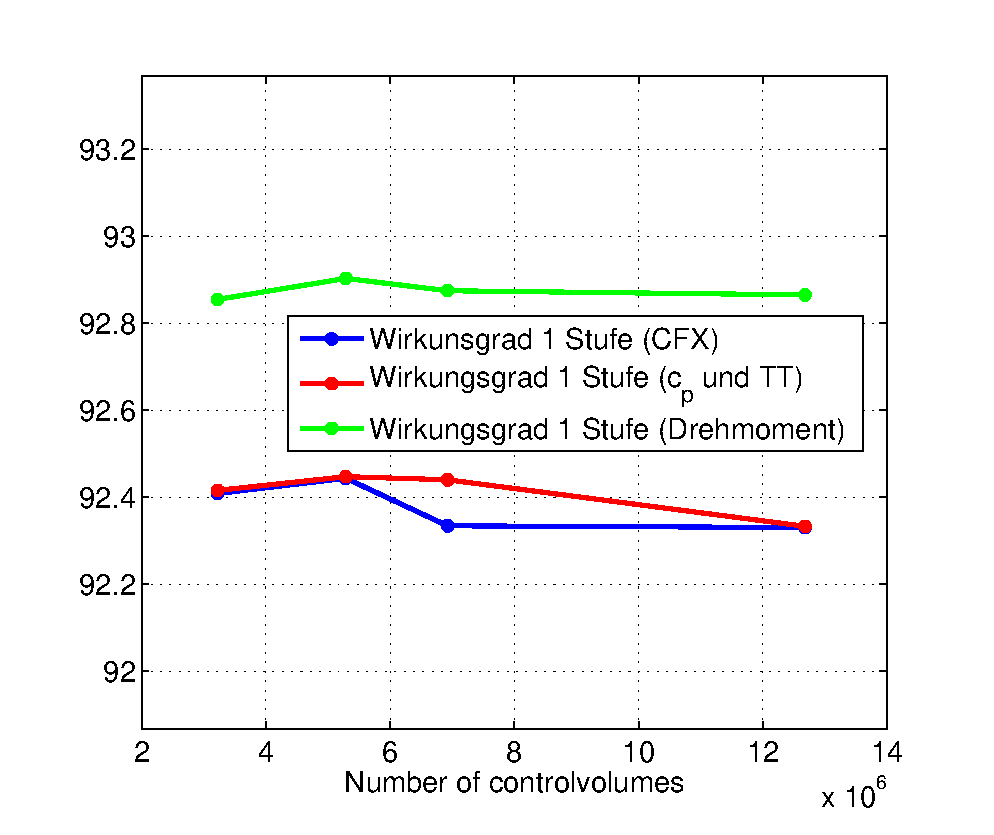
\includegraphics[width=0.7\textwidth]{efficiencies1strukturiert}
	\caption{Wirkungsgrade über eine Stufe} \label{fig:efficiencies1strukturiert}
\end{figure}

\begin{figure}[H]
	\centering
	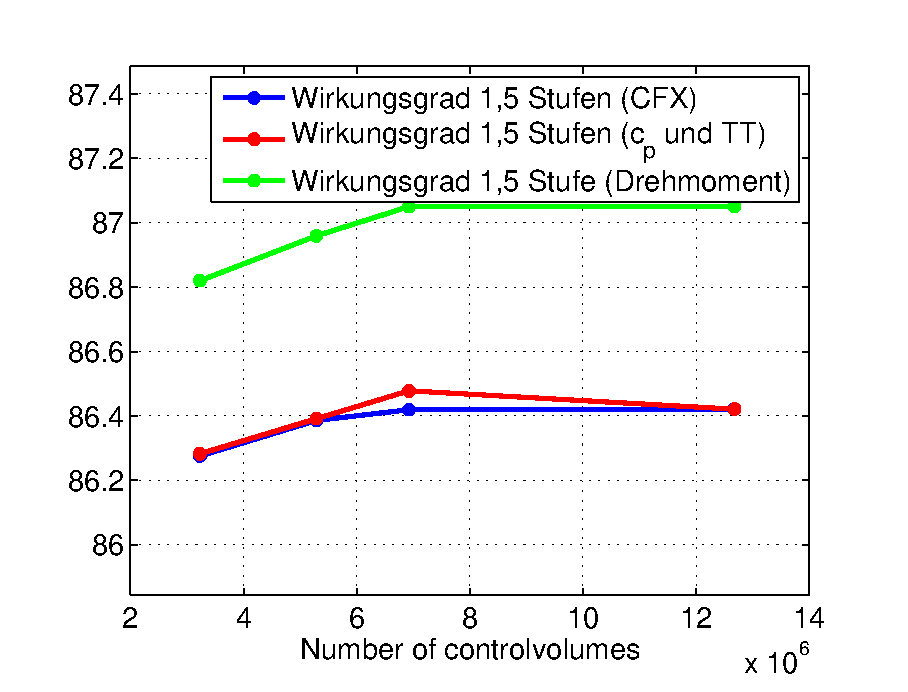
\includegraphics[width=0.7\textwidth]{efficiencies15strukturiert}
	\caption{Wirkungsgrade über 1,5 Stufen} \label{fig:efficiencies15strukturiert}
\end{figure}


\subsection{Fillets}

In realen Turbinen befinden sich an der Schaufel am Übergang zum Randbereich fertigungsbedingte Fillets, Verrundungen, um Ablöseblasen zu vermeiden und bessere Strömungs- und Festigkeitseigenschaften zu erzielen. Da außerdem die Qualität der Zellen am Übergang zur Nabe sehr schlecht war, wurde noch eine Simulation der Aachen-Turbine mit Fillets durchgeführt. Das Netz ist in Abb. \ref{imgFillet1} zu sehen. Jedoch ergab sich das Problem, dass nur sehr kleine Fillets erstellt werden konnten, da die Statoren eine „Delle“ an der Vorderkante aufweisen, wie in Abb. \ref{imgFilletDelle} zu sehen ist und daher ab einem bestimmten Filletradius negative Kontrollvolumen durch die Fillets entstehen. Deswegen wurde eine Simulation mit einem Fillet des Radius 0.00055 durchgeführt. Es hat sich herausgestellt, dass die Gitterqualität wesentlich schlechter wurde, da sich mehr schrägwinklige Zellen im Filletbereich befanden. Allerdings wurde der $y^+$-Wertebereich besser, da sehr kleine und sehr große Werte verschwanden.     

  \begin{figure}[H]
	\centering
	\includegraphics[width=0.7\textwidth]{fillet0_00055.png}
	\caption{Netz mit Fillet der Größe 0.00055} \label{imgFillet1}
\end{figure} 

  \begin{figure}[H]
	\centering
	\includegraphics[width=0.7\textwidth]{filletDelle.png}
	\caption{Delle in der Statorgeometrie} \label{imgFilletDelle}
\end{figure} 
\section{Unstrukturiertes Gitter}
Um generelle Unterschiede zwischen einem strukturierten und unstrukturierten Gitter festzustellen, wurden zusätzlich Berechnungen mit einem unstrukturierten Gitter durchgeführt.

\subsection{Aufgetretene Probleme}
Für den zweiten Stator liegt kein CAD-File, lediglich eine Netzdatei vor. Somit war es nicht möglich ein unstrukturiertes Gitter für diesen zu erstellen. Für die Berechnungen wurde daher das Gitter der Aachen-Turbine teilweise unstrukturiert und strukturiert betrachtet.\\
Die Erstellung der unstrukturierten Gitter war aufgrund von Lizenzproblemen nicht immer möglich, was die Anzahl der durchgeführten Simulationen eingrenzt.
\subsection{Erstellung des Gitters}
Das unstrukturierte Gitter wurde mit Centaur erstellt. Zunächst wurde ein Referenzgitter mit den Standardwerten gebildet. Für das Einstellen von $y^+$ wurde zunächst der gleiche Wandabstand wie im Falle des strukturierten Gitters verwendet. Nach einem ersten Test wurde dieser im Rotor verringert. Die Verteilung von $y^+$ des ersten Stators und Rotors ist in Abbildung \ref{yplusunstrukturiert} dargestellt.
\begin{figure}[htbp]
	\centering
	\includegraphics[width=0.7\textwidth]{yplusunstrukturiert.png}
	\caption{$y^+$ des unstrukturierten Gitters} \label{yplusunstrukturiert}
\end{figure}
\subsubsection{Verwendung von Sources}
Um das Gitter lokal an bestimmten Stellen zu verfeinern wurden  sogenannte Sources mit Hilfe Centaur eingeführt.
Eine davon regelt die unterschiedlichen Wandabstände von Schaufel, Nabe und Gehäuse.\\
Eine weitere Source verfeinert die Zellen im Nachlauf der Schaufel relativ zu den umliegenden Zellen um den Faktor $c = 0.8$.

\subsection{Gitterstudie}
Zuerst wurde der Spalt des Rotors wie beim strukturierten Gitter verfeinert. Anschließend wurde eine Gitterstudie mit verschiedenen Verfeinerungsstufen, siehe Tabelle \ref{tab:verfeinerungenunstrukturiert}, durchgeführt. In den Abbildungen \ref{fig:gitterunstrukturiert1stufe} und \ref{fig:gitterunstrukturiert15stufen} ist der Wirkungsgrad in \% über die Verfeinerungsstufen aufgetragen. Es ist zu erkennen, dass die Wirkungsgrade weiterhin in Abhängigkeit der Kontrollvolumenzahl steigen. Damit eine netzunabhängige Lösung ermittelt werden kann, müssten weitere Verfeinerungsstufen zwischen 2 und 3 und größer 3 gerechnet werden, bis kein Ansteigen oder Absinken mehr zu erkennen ist. Dies war aufgrund von Lizenzproblemen nicht möglich.\\
Für die Berechnungen mit einem temperaturabhängigen $c_p$ und für die Vergleiche mit dem strukturierten Gitter wurde das feinste Netz verwendet.
\begin{table}[h]
		\centering
		\caption{Verfeinerungsstufen des unstrukturierten Gitters}
	\begin{tabular}{ c| c | c| c| c}
Verfeinerungsstufe	&	Stator 1	&		&	Rotor	&		\\
&	Anzahl Knoten	&	Anzahl Elemente	&	Anzahl Knoten	&	Anzahl Elemente	\\
\hline									
0,5	&	61435	&	174098	&	281782	&	724470	\\
1	&	147399	&	473211	&	638948	&	1741931	\\
2	&	244772	&	880367	&	1007020	&	2835297	\\
\textbf{3}	&	\textbf{1196277}	&	\textbf{6457352}	&	\textbf{1880370}	&	\textbf{6844537}	\\

	\end{tabular}
		\label{tab:verfeinerungenunstrukturiert}
\end{table}
\begin{figure}[htbp]
	\centering
	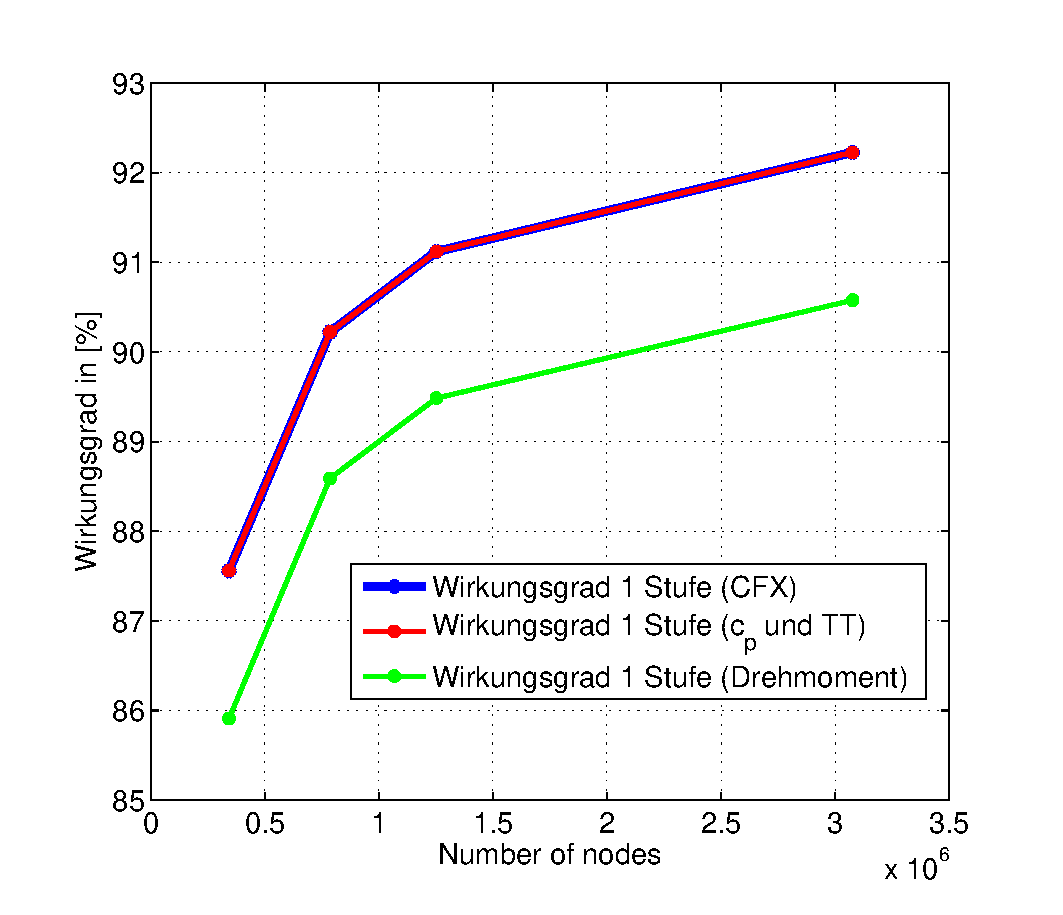
\includegraphics[width=0.7\textwidth]{gitterstudieunstrukturiert1stufe.eps}
	\caption{Gitterstudie des unstrukturierten Gitters für eine Stufe} \label{fig:gitterunstrukturiert1stufe}
\end{figure}

\begin{figure}[htbp]
	\centering
	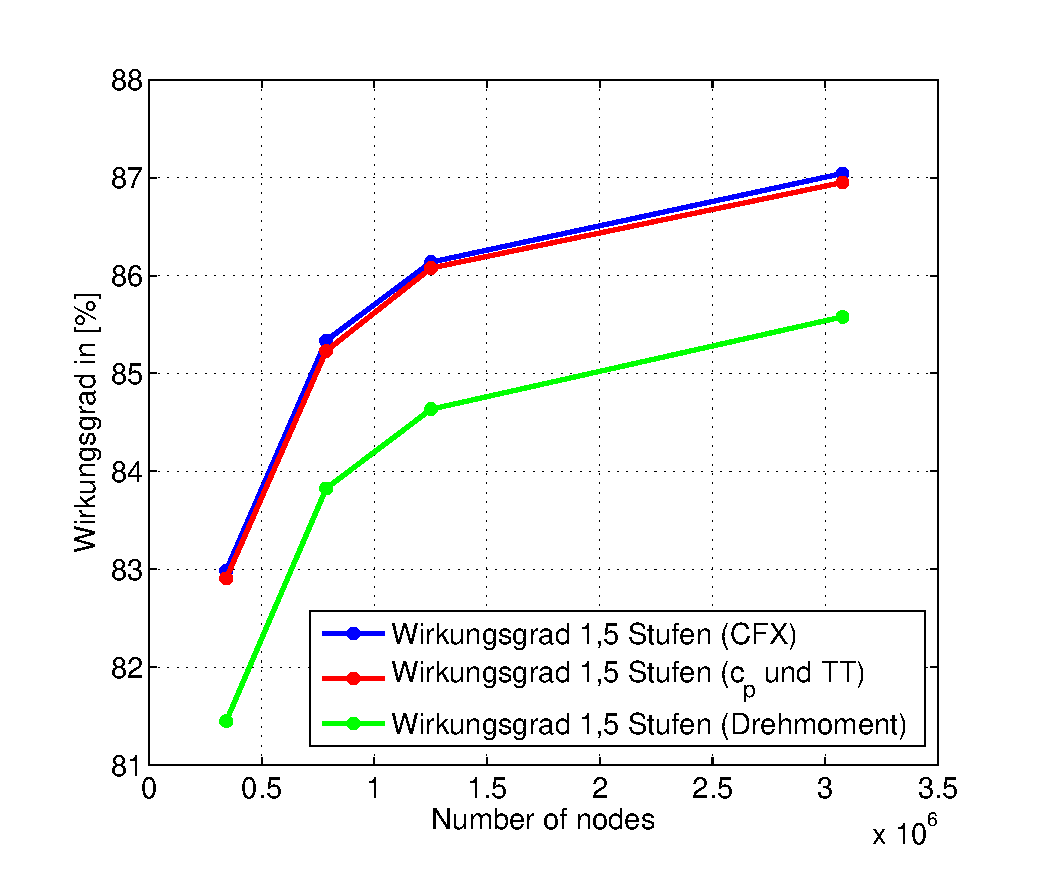
\includegraphics[width=0.7\textwidth]{gitterstudieunstrukturiert15stufen.eps}
	\caption{Gitterstudie des unstrukturierten Gitters für 1,5 Stufen}
	\label{fig:gitterunstrukturiert15stufen}
\end{figure}
\section{Vergleich der Wirkunsgrade}
Bei der Aachen-Turbine ergaben sich je nach Berechnungsart folgende Werte für den Wirkungsgrad:
\begin{table}[H]
	\centering
	\caption{Wirkungsgrad bei der Aachen-Turbine}
	\begin{tabular}{ c| c | c}
Berechnungsformel	&	$\eta_{strukturiert}$	&	$\eta_{unstrukturiert}$	\\
\hline
1 Stufe	&		&		\\
\hline
$\eta_{CFX}$	&	$92,33\%$	&	$92,23\%$	\\
$\eta_{c_p, T_t}$	&	$92,44\%$	&	$92,23\%$	\\
$\eta_{torque}$	&	$92,87\%$	&	$90,58\%$	\\
\hline
1,5 Stufen 	&		&		\\
\hline
$\eta_{CFX}$	&	$86,42\%$	&	$87,05\%$	\\
$\eta_{c_p, T_t}$	&	$86,48\%$	&	$87\%$	\\
$\eta_{torque}$	&	$87.05\%$	&	$85,58\%$	\\

	\end{tabular}
	\label{tab:wgaachen}
\end{table}
In Tabelle \ref{tab:wgaachen} werden die Wirkungsgrade des strukturierten und des unstrukturierten Gitters dargestellt. Diese weichen höchstens um $1,7\%$ voneinander ab. Es ist zu erkennen, dass die Wirkungsgrade im strukturierten Fall bei einer Stufe bis zu zwei Prozentpunkten größer sind. Bei der Betrachtung von 1,5 Stufen ist dagegen zu erkennen, dass die Wirkungsgrade im strukturierten Fall um $0,6$ Prozentpunkte kleiner sind.\\
Dies kann an dem Übergang vom Rotor in den zweiten Stator liegen. Dort findet ein Wechsel des Gitters von unstrukturiert nach strukturiert statt.\\
Allerdings ist die durchgeführte Gitterstudie im unstrukturierten Fall nicht zufriedenstellend durchgeführt, was in den Abbildungen \ref{fig:gitterunstrukturiert1stufe} und \ref{fig:gitterunstrukturiert15stufen} zu erkennen ist. Daher fällt ein Vergleich der beiden Gittertypen schwer und ist nicht aussagekräftig. \\ 

Aus den physikalischen Grundlagen zur Berechnung des Wirkungsgrades ist nach dem Satz der Massenerhaltung der Massenstrom über die gesamte Turbine konstant.
Aufgrund numerischer Faktoren, sowie konstruktionsbedingt kann es jedoch zu Veränderungen im Massenstrom kommen. 
Insbesondere kommt es an den Verbindungsstellen der einzelnen Domänen zu Abweichungen. Hierzu wird in Kapitel \ref{cha:kanal} näher eingegangen.
Auffällig ist jedoch, dass es hierbei gravierende Unterschiede im Hinblick auf die Gitterstrukturierung gibt. In Abbildung \ref{fig:massFlowUnstrukt} ist der Verlauf des Massenstroms durch die Turbine dargestellt. Die Position in der Turbine ist auf der Abszisse dargestellt, die Interfaces befinden sich bei 1 und 2. Auf der Ordinate ist der jeweilige Massenstrom aufgetragen. Für die unstrukturierte Vernetzung treten Massenstromunterschiede von $0,1664 \frac{kg}{s}$ auf. Im Vergleich dazu liegt die Massenstromabweichung für das strukturierte Gitter, siehe Abbildung \ref{fig:massFlowStrukt}, lediglich bei $0.00028\frac{kg}{s}$.

 \begin{figure}[htbp]
	\centering
	\includegraphics[width=0.8\textwidth]{massFlow_strukt.eps}
	\caption{Massenstrom über in der Turbine, strukturiertes Gitter} \label{fig:massFlowStrukt}
\end{figure} 
 \begin{figure}[htbp]
	\centering
	\includegraphics[width=0.8\textwidth]{massFlow_unstrukt.eps}
	\caption{Massenstrom über in der Turbine, unstrukturiertes Gitter} \label{fig:massFlowUnstrukt}
\end{figure} 
\subsection{Wirkungsgrade mit temperaturabhängigem $c_p$}
\begin{table}[H]
	\centering
	\caption{Vergleich der Wirkungsgraddefinitionen auf einem strukturierten Gitter mit $c_p = f(T)$}
	\begin{tabular}{ l| c | c c c c}
		&	$c_p = const.$	&	$c_p(T)$	&		&		&		\\
		\hline
		&		&	CpIs	&	Ave CpIS	&	Ave	&	mycp	\\
		\hline
		$\eta_{CFX}$	&	81,24 \%	&	53,89\%	&	79,19 \%	&	79,19 \%	&	60,25\%	\\
		$\eta_{c_p, T_t}$	&	81,25\%	&	74,6 \%	&	78,3 \%	&	78,07\%	&	83,41 \%	\\
	$\eta_{torque}$	&	82,52\%	&	54,35 \%	&	80,11 \%	&	79,87 \%	&	60,77\%	\\
		
	\end{tabular}
	\label{tab:strukturiertmycp}
\end{table}

\begin{table}[H]
	\centering
	\caption{Vergleich der Wirkungsgraddefinitionen auf einem unstrukturierten Gitter mit $c_p = f(T)$}
	\begin{tabular}{ l| c | c c c c}
		&	$c_p = const.$	&	$c_p(T)$	&		&		&		\\
		\hline
		&		&	CpIs	&	Ave CpIS	&	Ave	&	mycp	\\
		\hline
		$\eta_{CFX}$	&	80,21 \%	&	71,93 \%	&	77,96 \%	&	78,34 \%	&	60,01 \%	\\
		$\eta_{c_p, T_t}$	&	80,1 \%	&	\textcolor{red}{100,36} \%	&	78,23 \%	&	78,61\%	&	83,72 \%	\\
		$\eta_{torque}$	&	79,5 \%	&	70,23 \%	&	77,1 \%	&	77,48 \%	&	59,36 \%	\\
		
	\end{tabular}
	\label{tab:unstrukturiertmycp}
\end{table}
%%% Local Variables: 
%%% mode: latex
%%% TeX-master: "main"
%%% End: 


 %Dominik Keijo eingefügt
	\chapter{Einfluss inhomogener Randbedingungen und des Stator-Rotor Interface auf die Wirkungsgradbestimmung}
\label{cha:kanal}
Bei der Berechnung des Wirkungsgrades führen geringe Abweichungen der Totaltemperatur zu großen Änderungen des Wirkungsgrades. An dem Stator-Rotor Interface kommt es bei Wahl einer sogenannten Mixing-Plane zur stationären Berechnung zu einem Ansteigen der Totaltemperatur. In diesem Kapitel wird zunächst die Funktionsweise der Mixing Plane erläutert und die Ergebnisse der Analyse des Einflusses der Mixing Plane bei unterschiedlichen Einstrombedingungen vorgestellt.
%______________________________________________________
\section{Mixing Plane / Stage}
In dem verwendeten Setup der Aachenturbine werden die 1 1/2 Stufen in drei Domänen dargestellt. Hierbei kommt es zu einer Herausforderung; die Domänen müssen miteinander verbunden werden. Um dies zu bewerkstelligen, werden jeweils an den Verbindungsstellen von Stator zu Rotor und Rotor zu Stator sogenannte \textit{Interfaces} definiert.
Im Falle einer solchen Anordnung ist in CFX die \textit{General Connection} zu wählen, da sich rotierende an stationäre Domänen anschließen.\\
Eine Möglichkeit ein solches Interface mittels General Connection zu definieren ist das Frozen Rotor Interface. Hierbei bleibt die relative Orientierung der Komponenten über die gesamte Berechnung erhalten. 
Dieses Modell hat seine Vorteile bei großen Schwankungen der Strömungsgrößen in Umfangsrichtung.\\
Eine weitere Untergruppe der \textit{General Connection} in CFX ist das Stage- oder Mixing Plane-Interface, welches für die Erstellung des in dieser Arbeit verwendeten Setups eingesetzt wird. Hierbei werden die Strömungsgrößen an der Verbindungsstelle über den Umfang gemittelt.
Durch die Mittelung der Strömungsgrößen am Interface treten Vermischungsverluste auf. Laut ANSYS sind die hierbei entstehenden Verluste äquivalent zu den physikalischen Vermischungseffekten der zwischen Stator und Rotor und eines somit entstehenden Geschwindigkeitsprofils in entgegen der Strömungsrichtung. \cite{Sharcnet1}

%Quelle: \url{
%<<<<<<< HEAD
%TODO %${https://www.sharcnet.ca/Software/Ansys/17.0/en-us/help/cfx_mod/CACDIGEH.html} %$- 12.06.2017 %TODO
%=======
%\textcolor{red}{TODO %${https://www.sharcnet.ca/Software/Ansys/17.0/en-us/help/cfx_mod/CACDIGEH.html} %$- 12.06.2017 TODO}
%>>>>>>> f3c40cd8607ef731dd159d84270213c9c754ef68
%_____________________________________________________________________
\section{Rohrauschnitt}
\label{sec:kanalgeo}
Anstelle der Aachen-Turbine wurde für die Analyse des Stator-Rotor Interface ein Rohrausschnitt, geteilt in Stator und Rotor, berechnet, um den Einfluss des Interfaces auf die Strömungsgrößen in Hinblick auf die Wirkungsgradberechnung zu testen. Dabei wurden die Eintrittsbedingungen verändert und das Verhalten der Mixing-Plane unter unterschiedlichen Anströmbedingungen untersucht. In den folgendem Abschnitt wird zunächst das Rechengebiet näher beschrieben.
%________________________________________________________
\subsection{Problemgebiet}
\label{subsec:kanalproblemgebiet}
Die Geometrie des Rohrausschnitts mit Gitter ist in der Abbildung \ref{fig:kanalgebiet} zu sehen.
\begin{figure}[H]
\includegraphics[width=\textwidth]{kanalmitmesh.png}
\caption{Eine dreidimensionale Ansicht der vereinfachten Aachen-Turbine mit Gitter.}
\label{fig:kanalgebiet}
\end{figure}
Die vereinfachte Turbine besteht aus einem Stator und einem Rotor. An der Vorderseite befindet sich der Einstrom, an den Seiten jeweils periodische Randbedingungen, an der Rückseite ist der Ausstrom. Die Grenzen an der Ober- und Unterseite stellen Shroud und Hub dar und werden als Wandrandbedingungen repräsentiert. Stator und Rotor sind mit einem Interface verbunden. Das Verhältnis der Abmessungen dieses Rohrausschnitts entspricht den Größenverhältnissen der Aachen-Turbine und sind der Tabelle \ref{tab:kanalabmessungen} zu entnehmen.
\begin{table}[H]
\centering
\label{tab:kanalabmessungen}
\caption{Abmessungen der vereinfachten Turbine}
\begin{tabular}{ c| c| c| c}
 $d_a$&$d_i$&$L_x$&$\alpha$\\
\hline
$300mm$&$240mm$&$160mm$&$45^\circ$\\
\end{tabular}
\end{table}
mit dem Außendurchmesser $d_a$, dem Innendurchmesser $d_i$, der Länge in Axialrichtung $L_x$ und dem Ausschnittswinkel $\alpha$.
%________________________________________________________
\subsection{Gitterstudie}
\label{subsec:kanalgitterstudie}
Nach Festlegen der Geometrie wurde ein CAD-Modell und ein Gitter mit einem $y^+ \approx 1$ erstellt. Darauf folgte eine Gitterstudie , um die Unabhängigkeit der Lösung von der Gitterdiskretition sicherzustellen. Dabei wurde das Rechengebiet auf immer feiner werdenden Gittern berechnet, bis sich die relevanten Größen nicht mehr verändert haben. In der folgenden Tabelle \ref{tab:kanalgitter} werden die Gitterparameter des Gitters gezeigt, die aus der Gitterstudie ermittelt und für die Analyse verwendet wurden. 
\begin{table}[H]
\centering
\caption{Gitterparameter des Kanals}
\begin{tabular}{ c| c| c| c| c}
$N_x$&$N_r$&$N_\phi$&Gesamtanzahl Knoten&Gesamtanzahl KV\\
\hline
48&56&79 &424704&403260\\
\end{tabular}
\label{tab:kanalgitter}
\end{table}
Dabei sind $N_x$, $N_r$ und $N_\phi$ die Anzahl an Knoten in die verschiedenen Raumrichtungen in Zylinderkoordinaten.\newline
Anschließend wurden für dieses Gitter Strömungssimulationen mit unterschiedlichen Eintrittsrandbedingungen und Veränderungen des Stator-Rotor Interfaces durchgeführt, die in dem folgendem Abschnitt beschrieben werden.

%_____________________________________________________________________________
\section{Einfluss des Stator-Rotor Interface auf den Wirkungsgrad}
\label{kanaleinfluss}
In diesem Abschnitt werden die unterschiedlichen verwendeten Eintrittsrandbedingungen näher erläutert und dann die Ergebnisse der verschiedenen Simulationen vorgestellt.
\subsection{Verwendete Eintrittsrandbedingungen}
\label{subsec:kanalrandbedingungen}
Bei dem Stator-Rotor Interface werden die Werte an den Knoten vor dem Interface nach Mittelung und Interpolation auf die Knoten nach dem Interface übertragen. Bei gleichem Gitter für Stator und Rotor können diese direkt zugeordnet werden. Deswegen wurde für einen Testfall das Gitter im Rotor verfeinert, sodass die Zuordnung der Knoten interpolativ erfolgen muss.\newline
Desweiteren wurde der Einfluss der Einstromrandbedingung in Bezug auf die Mixing Plane ermittelt. Dabei wurde eine schräge Einströmung (Abbildung \ref{fig:randbedingungen}\subref{subfig-2:randbedingungen}), eine inhomogene Temperaturverteilung mit maximaler Temperatur in Rechengebietsmitte (Abbildung \ref{fig:randbedingungen}\subref{subfig-3:randbedingungen}/\subref{subfig-4:randbedingungen}) und schließlich zusätzliche Dralleintrittsrandbedingungen mit unterschiedlicher Drallkernposition (Abbildung \ref{fig:randbedingungen}\subref{subfig-5:randbedingungen}/\subref{subfig-6:randbedingungen}) vorgegeben.
\begin{figure}[htbp]
\centering
%\subfigure[Feineres Gitter im Rotor]{\includegraphics[width=0.45\textwidth]{bilder/feinererrotor.png}\label{subfig-1:randbedingungen}}
\subfigure[Schräger Strömungseintritt]{\includegraphics[width=0.8\textwidth]{schraegeStromlinien_Vector.png}\label{subfig-2:randbedingungen}}
\subfigure[Inhomogene $T_t$ (vor Interface)]{\includegraphics[width=0.45\textwidth]{TtVorMP.png}\label{subfig-3:randbedingungen}}
\subfigure[Inhomogene $T_t$ (nach Interface)]{\includegraphics[width=0.45\textwidth]{TtNachMP.png}\label{subfig-4:randbedingungen}}
\subfigure[DralleintrittsRB A]{\includegraphics[width=0.45\textwidth]{drallkernA.png}\label{subfig-5:randbedingungen}}
\subfigure[DralleintrittsRB B]{\includegraphics[width=0.45\textwidth]{drallkernb.png}\label{subfig-6:randbedingungen}}
\caption{Verwendete Randbedingungen}
\label{fig:randbedingungen}
\end{figure} 
Anstatt nur stationär mit einer Mixing Plane wurde die Berechnung auch vollständig instationär mit einer Sliding Plane durchgeführt. Die Ergebnisse dieser Berechnungen werden im nächsten Abschnitt vorgestellt.
\subsection{Einfluss auf die Strömungsgrößen}
\label{subsec:kanalrandbedingungen}
Zur Untersuchung des Stator-Rotor Interface wurden die Strömungsgrößen vor und nach dem Interface miteinander verglichen, indem die Differenz nach
\begin{equation}
\label{eq:tdifferenz}
\Delta T_{t} = T_{t,2} - T_{t,1}
\end{equation}
berechnet wurde, wobei $T_{t,1}$ die Totaltemperatur vor dem Interface und $T_{t,2}$ die Totaltemperatur nach dem Interface ist. Dabei ergibt sich folgende Tabelle \ref{tab:kanalbedingungen} mit den Strömungsgrößen Massenstrom $\dot m$, Totaldruck $p_t$ und Totaltemperatur $T_t$.
\begin{table}[H]
\centering
\caption{Einfluss der Eintrittsrandbedingungen}
\begin{tabular}{ c| c| c| c}
Einstromrandbedingung& $\Delta \dot m$ in $\frac{kg}{s}$ & $\Delta p_t$ in $Pa$ &  $\Delta T_t$ in $K$\\%&$\Delta \eta$\\
\toprule
Referenzlösung&+1,252e-05&-40,04&+0,043\\%&+0,15\%\\
feineres Gitter im Rotor&+3,755e-06&-43,81&+0,043\\%&+0,15\%\\
schräge Einströmung&-7,368e-06&-35,45&+0,026\\%&-0,04\% \\
inhomogene TemperaturRB&+1,078e-06&+10,36&+0,794\\%&+2,29\% \\
DralleintrittsRB A&-1,051e-05&-38,59&+1,764\\%&+5,45\% \\
DralleintrittsRB B&-1,312e-05&-41,83&+1,632\\%&+5,04\% \\
DralleintrittsRB C&-8,919e-06&-93,04&+1,719\\%&+5,12\% \\
DralleintrittsRB D&-1,539e-05&+2,787&+1,597\\%&+5,11\% \\
DralleintrittsRB E&+4,091e-06&-12,07&+1,576\\%&+4,99\% \\
DralleintrittsRB F&+1,729e-06&-23,83&+1,626\\%&+5,10\% \\
\midrule
Instationär&+1,873e-07&-0,604&-2,466e-04\\%&+0\% \\
\end{tabular}
\label{tab:kanalbedingungen}
\end{table}
Es ist zu sehen, dass die Massenströme vor und nach dem Stator-Rotor Interface für alle Einstrombedingungen annähernd gleich groß sind. Der Totaldruck sinkt um bis zu maximal $\Delta P_{t_{max}} \approx 93 Pa$ und somit ist der Totaldruckverlust im Vergleich zu den vorherrschenden Totaldrücken $\frac{\Delta p_t}{p_t} \approx 10^{-4}$ klein. \newline Die Totaltemperatur ändert sich bei homogenen Temperaturrandbedingungen sowohl für schräge Einströmungsrandbedingungen als auch bei feinerem Gitter im Rotor kaum ($\Delta T_t < 0,05 K$). \newline
Bei inhomogenen Temperaturrandbedingungen unterscheidet sich die Totaltemperatur vor und nach dem Interface um ungefähr $\Delta T_t \approx 0,8K$. Hier ist der Unterschied von $T_t$ im Vergleich zum vorher homogenen Temperaturfeld wesentlich größer. Insbesondere bei zusätzlichen Dralleintrittsbedingungen ergeben sich Totaltemperaturdifferenzen von bis zu $\Delta T_t \approx 1,8K$. Bei Dralleintrittsbedingungen mit inhomogenen Randbedingungen sind somit die Abweichung der Totaltemperatur ungefähr doppelt so hoch wie bei keinen Dralleintrittsrandbedingungen (und nur inhomogenen Temperaturfeld).\\
Die Untersuchung der Mixing Plane erfolgte mit einer vereinfachten Turbine ohne Schaufeln. Bei diesem Fall wird im Rotor ohne Schaufeln keine Leistung erzeugt, sondern der Strömung Energie durch Rotation und Reibung zugeführt. Dies hat zur Folge, dass bei diesem Problemgebiet direkt keine Aussagen über den Wirkungsgrad wie bei einer Turbine getroffen werden kann. Um dennoch zumindestens eine grobe Abschätzung der Veränderung des Wirkungsgrades durch die Mixing Plane zu erhalten, wurden die Ergebnisse für $\Delta p_t$ und $\Delta T_t$ für diese Geometrie auf die Aachen Turbine übertragen. Dabei wurde die Aachen Turbine mit dem gleichen Betriebspunkt wie die vereinfachte Rohrströmung gerechnet und die Differenzen an den beiden Interfaces Stator1-Rotor und Rotor-Stator2 betrachtet. Diese Differenzen wurden dann bei der Wirkungsgradberechnung eliminiert, um einen korrigierten Wirkungsgrad zu berechnen (frei von den Differenzen an der Mixing Plane). Auf diesen korrigierten Wirkungsgrad wurden dann die Differenzen, die sich bei der vereinfachten Rohrströmung ergeben haben, wieder aufaddiert, unter der Annahme, dass sich die Aachen Turbine bei unterschiedlichen Eintrittsbedingungen ähnlich wie die Rohrströmung verhält. Damit ergaben sich folgende Abweichungen des Wirkungsgrads $\Delta \eta$ durch die Mixing Plane:
\begin{table}[htbp]
\centering
\caption{Abschätzung des Einflusses der MP auf den Wirkungsgrad}
\begin{tabular}{ c| c}
Einstromrandbedingung&$\Delta \eta$\\
\toprule
Referenzlösung&-0,264\%\\
feineres Gitter im Rotor&-0,274\%\\
schräge Einströmung&-0,190\% \\
inhomogene TemperaturRB&-2,775\% \\
DralleintrittsRB A&-6,345\% \\
DralleintrittsRB B&-5,884\% \\
DralleintrittsRB C&-6,343\% \\
DralleintrittsRB D&-5,629\% \\
DralleintrittsRB E&-5,599\% \\
DralleintrittsRB F&-5,808\% \\
\midrule
Instationär&$-8 \cdot 10^{-4}\%$ \\
\end{tabular}
\label{tab:kanalwg}
\end{table}
Hierbei ist jedoch anzumerken, dass aufgrund der vielen Annahmen diese Abschätzung nicht als allgemeine Aussage für die Wirkungsgradbestimmung zu sehen ist, sondern nur eine grobe Abschätzung der Größenordnung des Einflusses der Mixing Plane darstellt.
%TO DO
FAZIT FAZIT
Die Berücksichtung des Einflusses der Mixing Plane für die Wirkungsgradbestimmung ist unerlässlich, sobald inhomogene Temperaturfelder an dem Interface auftreten. Hier sollten die Domains instationär mit einer Sliding Plane verbunden werden, um die Verfälschung der Strömung durch Mittelung an der Mixing Plane zu vermeiden. Außerdem ist hier zu erwähnen, dass in diesem Testfall nur der Einfluss eines einzelnen Interfaces untersucht wurde. Bei einer Simulationen von mehreren Turbinenstufen und somit der Verwendung von mehreren Interfaces summiert sich der Fehler am Interface.

%%% Local Variables: 
%%% mode: latex
%%% TeX-master: "main"
%%% End: 


 %Dominik Keijo eingefügt
	\chapter{Auswertungstool zur Gitterstudie}
\todo
	
	
	\listoffigures			            		             % Abbildungsverzeichnis
	\addcontentsline{toc}{chapter}{Abbildungsverzeichnis}
	\listoftables                                    % Tabellen Verezeichnis
	\addcontentsline{toc}{chapter}{Tabellenverzeichnis}
	\bibliographystyle{plainnat}   			             % gibt den Stil des Literaturverzeichnises 
	\bibliography{literatur}     		             % Literaturverzeichnis
	\addcontentsline{toc}{chapter}{\bibname}         % hinzufügen ins Inhaltsverzeichnis
\end{document} 

